\chapter{General Description}

\section{System Architecture}

The Unicity protocol employs a hierarchical three-layer architecture designed for scalability and decentralization. Each layer serves a distinct function in the system:

\begin{figure}[!htbp]
    \centering
        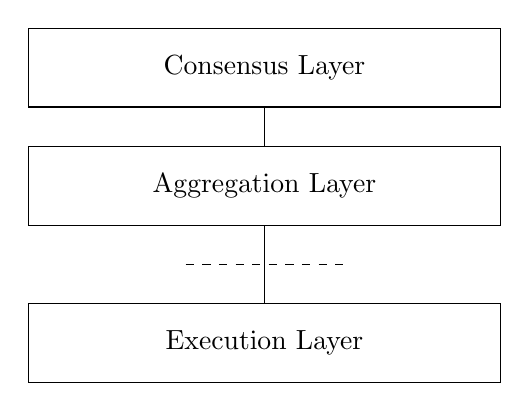
\begin{tikzpicture}
            \draw (0,0) rectangle (6,1) node[midway] {Consensus Layer};
            \draw (3,0) -- (3,-0.5);
            \draw (0,-1.5) rectangle (6,-0.5) node[midway] {Aggregation Layer};
            \draw[dashed] (2,-2) -- (4,-2);
            \draw (3,-1.5) -- (3,-2.5);
            \draw (0,-3.5) rectangle (6,-2.5) node[midway] {Execution Layer};
        \end{tikzpicture}
    \caption{Hierarchical architecture of the Unicity Network.}\label{fig:unicity-layers}
\end{figure}

\begin{description}
\item[Consensus Layer] PoW chain and BFT Core. Provides token minting, decentralized agreement and finality through Byzantine Fault Tolerant consensus. This layer verifies the integrity of the Aggregation Layer's state transitions and serves as the root of trust for the entire system. The BFT Core certifies SMT root hashes submitted by the aggregation layer.

\item[Aggregation Layer] Maintains a global append-only registry of spent token states using sharded Sparse Merkle Trees (SMT). Each partition within this layer processes state certification requests, provides inclusion proofs, and uses consistency proofs to enable trustless verification. The layer is organized into partitions for service design flexibility, with each partition potentially divided into shards for horizontal scalability.

\item[Execution Layer] Handles off-chain transaction processing and business logic. Token transactions occur peer-to-peer between users, with only cryptographic commitments to state transitions submitted to the Aggregation Layer for certification. This design moves computational overhead off-chain while maintaining trustless double-spending prevention.
\end{description}

The BFT Core certifies state transitions by cryptographically signing the root hashes of the Aggregation Layer's SMTs. This hierarchical design enables linear scalability: the BFT Core's throughput requirements grow only with the number of shards, not with the number of transactions processed by the system.
